% !TeX spellcheck = de_DE

%  ******************************************************************************
%  * @file      tex/Grundlagen                                                  *
%  * @author    Mario Hesse                                                     *
%  * @version   v0.1.1                                                          *
%  * @date      16.10.2019                                                      *
%  ******************************************************************************

\clearpage

\section{Grundlagen}

Hier sollten alle Themen erklärt werden, die zum Verständnis für die Arbeit nötig sind. In diesem Kapitel werden beim Leser die theoretischen Grundlagen gelegt, mit denen er den Rest der Arbeit verstehen kann. Fachbücher \citep{Helmke2016,Metelmann2016} sind in diesem Kapitel die bevorzugte Literatur. 

Gute Bilder helfen komplexe Inhalte leichter zu verstehen und geben einen schnellen ersten Eindruck. Daher sollte man in der gesamten Arbeit möglichst viele aussagekräftige Bilder verwenden. \autoref{pic:EinErstesBild} ist ein Beispiel dafür.

\begin{figure}[htbp]
	\centering
	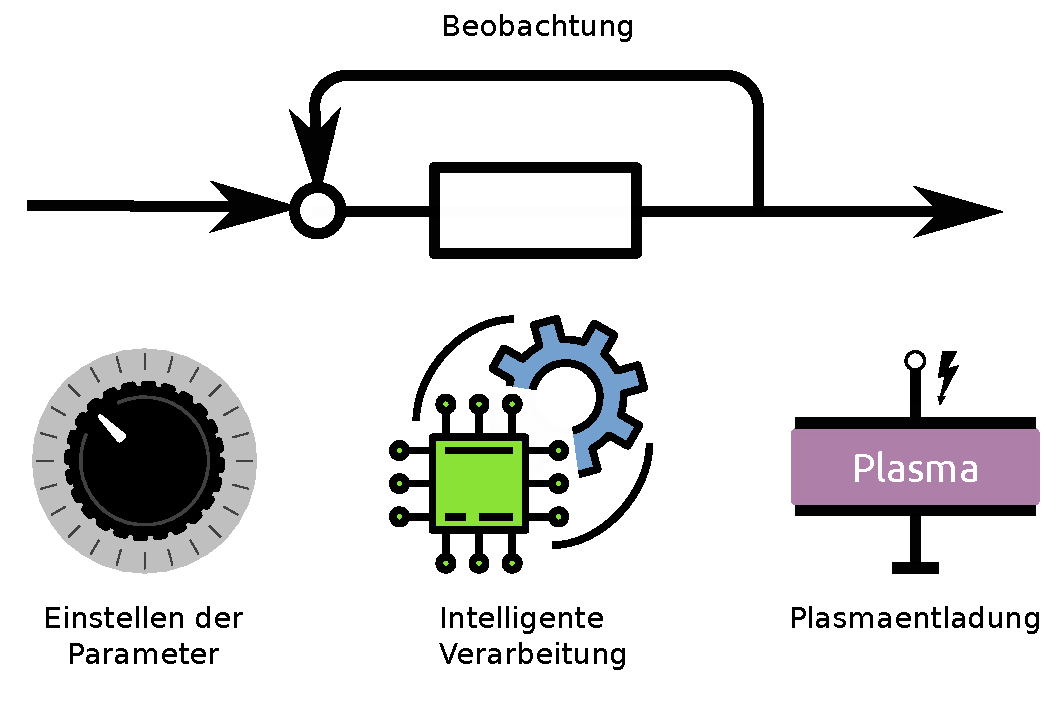
\includegraphics[width=0.5\linewidth]{pic/IntelligentesPlasma.pdf}
	\caption{Ein erstes Bild}
	\label{pic:EinErstesBild}
\end{figure}
